% --------------------------------------
%
% XMEN Lab.
% BlockGuide Template Documentation
%
% --------------------------------------

%----------------
% Packages configuration
%----------------
\documentclass[a4paper]{article}

\usepackage[a4paper, left=2.5cm, right=2cm]{geometry} % A4 paper size and thin margins
\usepackage[table,xcdraw]{xcolor} % Required for specifying custom colours

\definecolor{grey}{rgb}{0.9,0.9,0.9} % Colour of the box surrounding the title
\definecolor{LightBlue}{rgb}{0.69,0.768,0.95} % Colour of the box surrounding the title

\usepackage[utf8]{inputenc} % Required for inputting international characters
\usepackage[T1]{fontenc} % Output font encoding for international characters
%\usepackage[sfdefault]{ClearSans} % Use the Clear Sans font (sans serif)
\usepackage{XCharter} % Use the XCharter font (serif)
\usepackage{graphicx}
\usepackage{draftwatermark} % adds draft watermark

\SetWatermarkLightness{0.85}
\SetWatermarkText{Confidencial}
\SetWatermarkScale{0.7}

\usepackage[owncaptions]{vhistory}
\usepackage{indentfirst}
\usepackage{longtable}

\usepackage{fancyhdr}
\pagestyle{fancy}
\rhead{\leftmark}
\lhead{Block Guide: XCGen}

\usepackage[portuguese]{babel}
\usepackage{adjustbox}
\usepackage{multirow}
\usepackage{listings}
\usepackage{tikz-timing} % timing diagram (waveforms)

\usepackage{blindtext}

\usepackage{hyperref}

\usepackage[T1]{fontenc}
\usepackage[utf8]{inputenc}

\usepackage{float} % Fix de tabelas flutuantes

%solução para centering de tabelas com colunas de largura fixa
\usepackage{array}
\newcolumntype{P}[1]{>{\centering\arraybackslash}p{#1}}
\newcolumntype{M}[1]{>{\centering\arraybackslash}m{#1}}

\hypersetup{
    colorlinks=true,
    linkcolor=black,
    filecolor=magenta,
    urlcolor=black,
    bookmarks=true,
}
\usepackage{listings}
\usepackage{color}

\definecolor{dkgreen}{rgb}{0,0.6,0}
\definecolor{gray}{rgb}{0.5,0.5,0.5}
\definecolor{mauve}{rgb}{0.58,0,0.82}

\lstset{frame=tb,
   language=C,
   aboveskip=3mm,
   belowskip=3mm,
   showstringspaces=false,
   columns=flexible,
   basicstyle={\small\ttfamily},
   numbers=none,
   numberstyle=\tiny\color{gray},
   keywordstyle=\color{blue},
   commentstyle=\color{dkgreen},
   stringstyle=\color{mauve},
   breaklines=true,
   breakatwhitespace=true
   tabsize=3
   }

\begin{document}

%----------------
% CAPA
%----------------
\begin{titlepage}

% Figures
\begin{figure}
\centering

\begin{minipage}{0.45\textwidth}
    \centering
    
\includegraphics[width=0.9\textwidth]{images/logo.jpg}
\end{minipage}\hfill
\begin{minipage}{0.45\textwidth}
    \centering
    
\includegraphics[width=0.9\textwidth]{images/logo_virtus.png}
\end{minipage}

\end{figure}

% Block name
\vspace{8cm}
\parbox[t]{0.93\textwidth}{ 
\parbox[t]{0.91\textwidth}{
    \centering
    \fontsize{36pt}{40pt}\selectfont
    \vspace{3cm}
    
    % Configure your block name here (<Block Name>):
    \textbf{XCGen \\
    Block Guide}
    
    \vspace{1.5cm}}
}
\end{titlepage}

% Confidential msg    
\pagebreak
\hspace{0pt}
\vfill
\begin{center}
\hfill\rule{\linewidth}{1pt} \\[4pt]
    Este é um documento \textbf{CONFIDENCIAL} \\
    é vetado qualquer reprodução ou divulgação não autorizada.\\[4pt]
    \hfill\rule{\linewidth}{1pt} \\[4pt]
\end{center}
\vfill
\hspace{0pt}
\pagebreak


%----------------
% VERSÕES
%----------------

\renewcommand \vhAuthorColWidth{.8\hsize}
\renewcommand \vhChangeColWidth{1.2\hsize}

\renewcommand{\vhhistoryname}{Histórico de Revisão}
\renewcommand{\vhversionname}{Versão}
\renewcommand{\vhdatename}{Data}
\renewcommand{\vhauthorname}{Autor(es)}
\renewcommand{\vhchangename}{Descrição}

\begin{versionhistory}
  \vhEntry{0.1}{28/10/20}{Marcio Almeida}{Versão inicial}
\end{versionhistory}


\newpage
\tableofcontents
\newpage

%----------------
% CAPITULOS
%----------------
\section{Prefácio} % (fold)
\label{sec:prefácio}
 Este documento apresenta informações sobre o projeto XCGen e seus blocos, utilizados no laboratório X-Men.
 Este documento não tem como objetivo dispensar a leitura e entendimento das especificações que são fornecidas pelos desenvolvedores.

\subsection{Convenções}

\begin{table}[H]
  \centering
  \renewcommand\arraystretch{1.25}
  \caption{Lista de convenções.}
  \vspace{0.3cm}
  \begin{tabular}{|P{2.5cm}|P{10.5cm}|}
    \hline
    \textbf{Convenção} & \textbf{Descrição} \\ \hline
    I                  & Quando aparece na coluna \textbf{I/O} em tabelas de descrição de sinais, significa que o sinal é uma entrada do módulo. \\ \hline
    O                  & Quando aparece na coluna \textbf{I/O} em tabelas de descrição de sinais, significa que o sinal é uma saída do módulo. \\ \hline
  \end{tabular}
\end{table}
\subsection{Contatos para correções ou dúvidas}
\begin{itemize}
\item marcio.almeida@embedded.ufcg.edu.br
\end{itemize}
\subsection{Bibliografia} % (fold)

Para maiores informações sobre qualquer um dos blocos, os links podem ser encontrados nos documentos a seguir:
\begin{itemize}
\item \url{http://www.gstitt.ece.ufl.edu/courses/fall15/eel4720_5721/labs/refs/AXI4_specification.pdf}
\item \url{https://riscv.org/technical/specifications/}
\item \url{https://en.wikipedia.org/wiki/JTAG}
\end{itemize}
\label{sub:bibliografia}

% subsection bibliografia (end)
\newpage
\subsection{Acrônimos e abreviações} % (fold)
% ######## init table ########
\begin{table}[h]
  \centering
  % distancia entre a linha e o texto
      {\renewcommand\arraystretch{1.25}
        \caption{Acrônimos e abreviações.}
        \vspace{0.3cm}
        \begin{tabular}{ l l }
          \cline{1-1}\cline{2-2}  
          \multicolumn{1}{|p{3.850cm}|}{\textbf{Acrônimo} \centering } &
          \multicolumn{1}{p{8cm}|}{\textbf{Significado} \centering }
          \\  
          \cline{1-1}\cline{2-2}  
          \multicolumn{1}{|p{3.850cm}|}{AXI4 \centering } &
          \multicolumn{1}{p{8cm}|}{{\it Advanced Extensible Interface} (
Interface Extensível Avançada) \centering }
         \\  
          \cline{1-1}\cline{2-2}  
          \multicolumn{1}{|p{3.850cm}|}{JTAG \centering } &
          \multicolumn{1}{p{8cm}|}{{\it Joint Test Action Group} (Grupo de ação de teste conjunto
) \centering }
\\
         \cline{1-1}\cline{2-2}  
          \multicolumn{1}{|p{3.850cm}|}{RISC \centering } &
          \multicolumn{1}{p{8cm}|}{{\it Reduced Instruction Set Computer} (Computador com um conjunto reduzido de instruções
) \centering }
\\
         \cline{1-1}\cline{2-2}  
          \multicolumn{1}{|p{3.850cm}|}{XCGen \centering } &
          \multicolumn{1}{p{8cm}|}{{\it Xmen Campina Grande Generator} (Gerador de SoC Desenvolvido em Campina Grande, no laboratório Xmen
) \centering }
     
          \\  
          \hline
          
      \end{tabular} }
\end{table}



\label{sub:acrônimos_e_abreviações}


%\vspace{4cm}
% subsection acrônimos_e_abreviações (end)




% subsection glossário (end)

\section{Introdução} % (fold)
\label{sec:introdução}

\begin{figure}[!htb]
  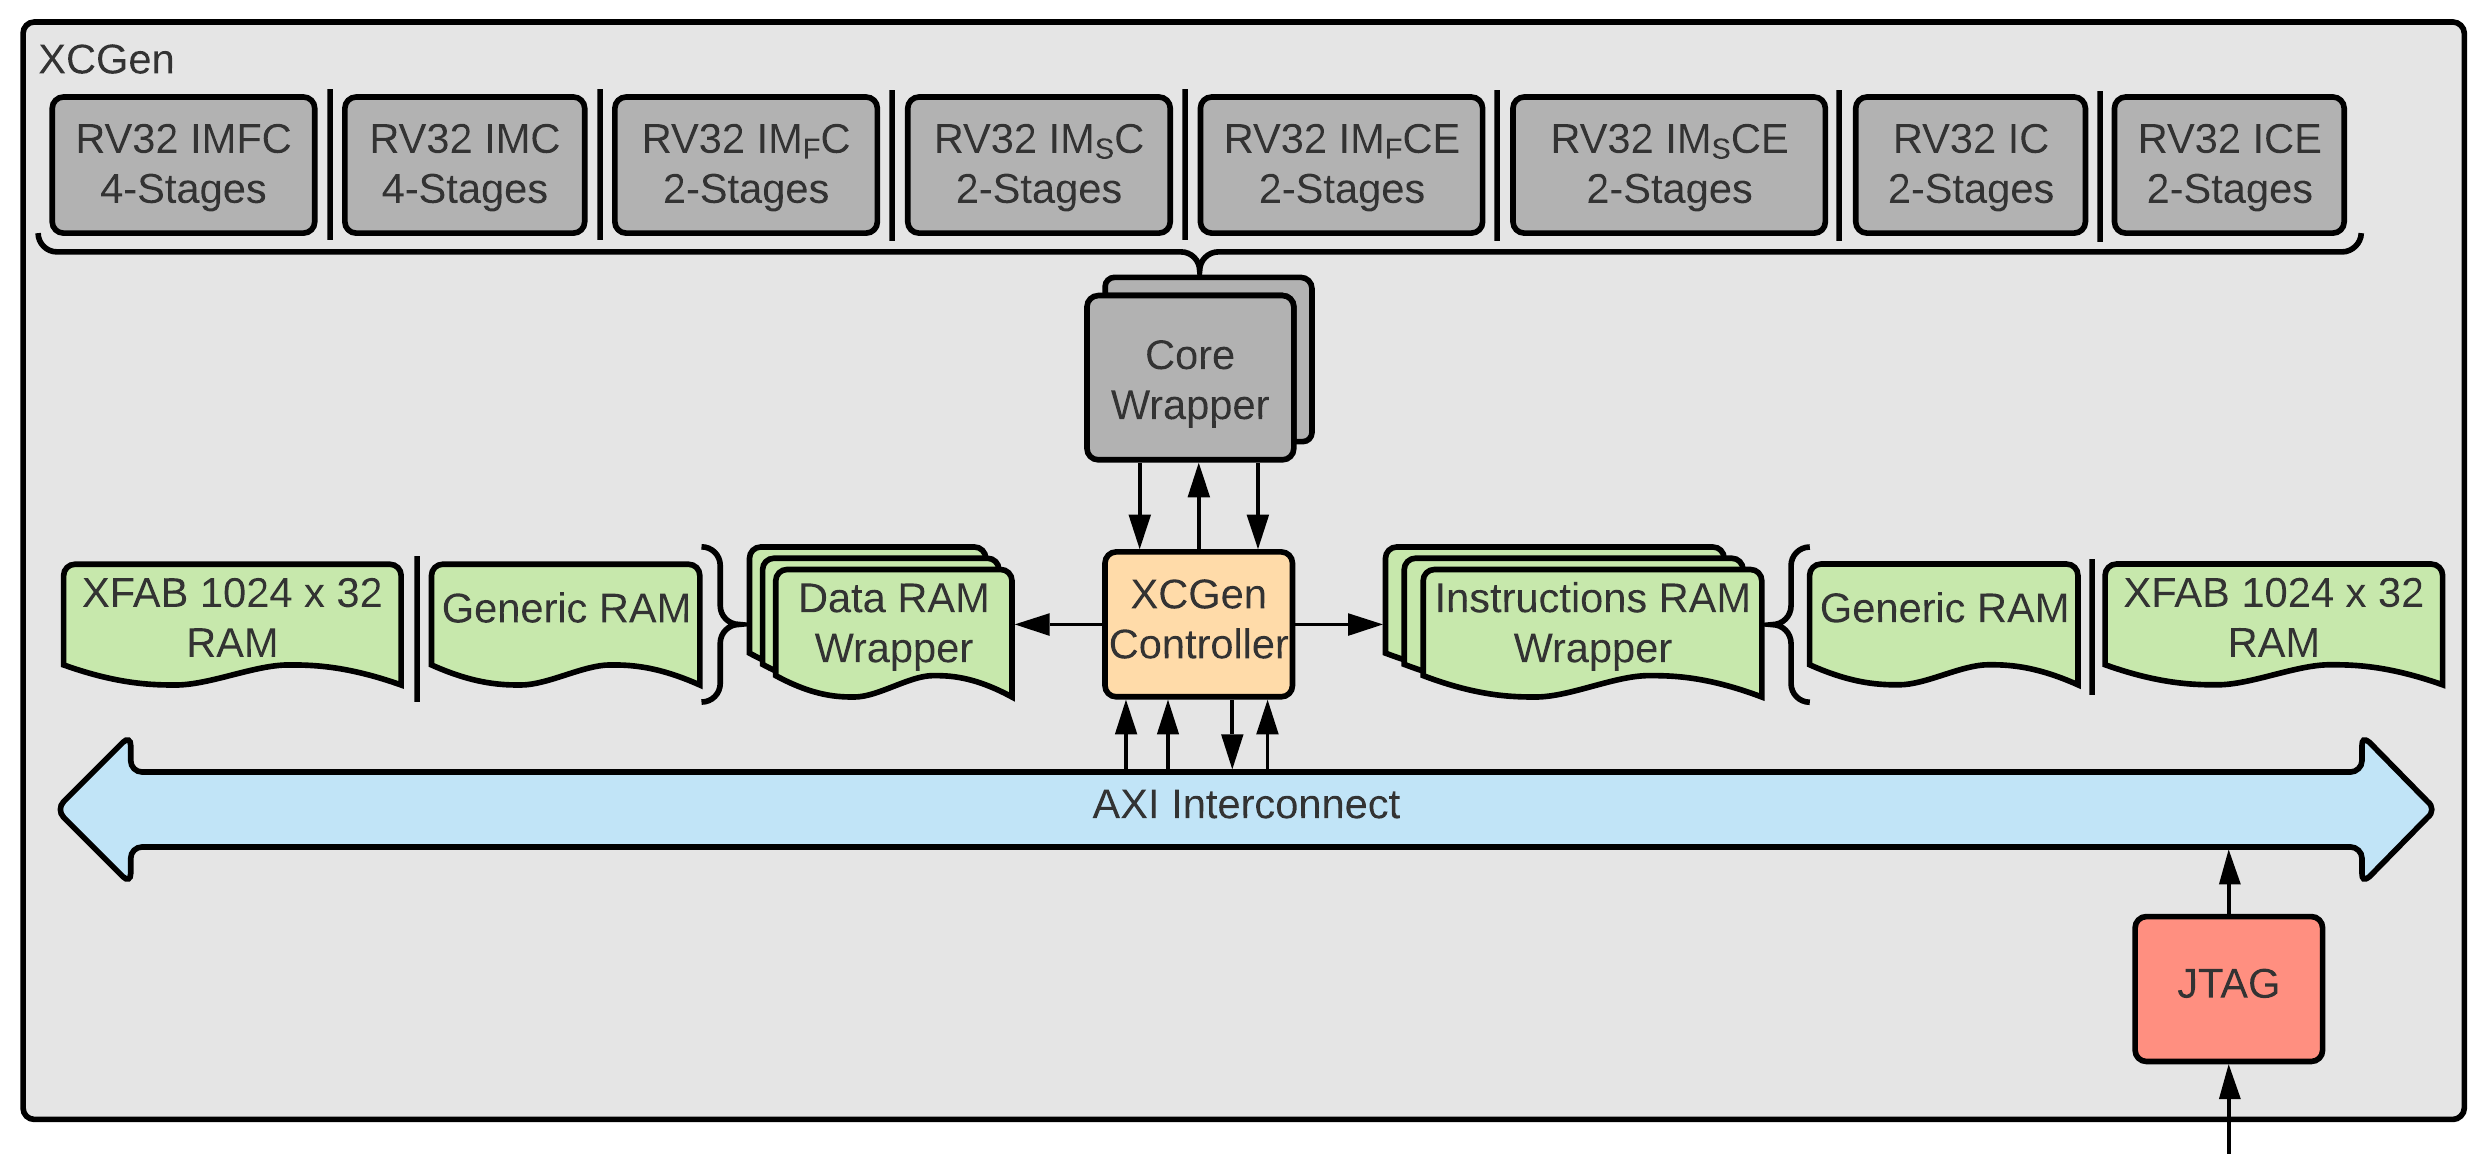
\includegraphics[width=\linewidth]{diagrams/XCGen2.png}
  \caption{Diagrama do XCGen.}
  \label{fig:top}
\end{figure}

\subsection{Visão Geral}
\label{sec:vgeral}
\par O XCGen consiste de um topo, feito na linguagem "System Verilog", onde é possível, através do uso de generates, adicionar ou remover blocos e alterar o mapa de memória na região de parametros do código.
Permitindo assim se ter novas funcionalidades e aplicações, através de um mesmo código, com o mínimo de alterações;
 \\
\par A arquitetura foi baseada no PULPINO o que permite o XCGen utilizra da ToolChain do RISC-V para geração de instruções em alto nível;

% section introdução (end)


\newpage

\section{Descrição dos sinais da interface} % (fold)
\label{sec:descrição_detalhada_de_sinais}

\subsection{Interface de Controle}
\label{sec:if_controle}

\begin{table}[H]
  \centering
  \renewcommand\arraystretch{1.25}
  \caption{Sinais de interface de controle detalhados.}
  \vspace{2mm}
  \begin{tabular}{|P{4.0cm}|P{0.7cm}|P{1.5cm}|P{8cm}|}
    \hline
    \textbf{Sinal}        & \textbf{I/O} & \textbf{Tamanho} & \textbf{Descrição}                                    \\ \hline
    clk\_i                 & I            & 1                & Clock síncrono                                       \\ \hline
    rst\_ni                & I            & 1                & Reset assíncrono baixo ativo                         \\ \hline
    test\_en\_i            & I            & 1                & Chaveia todos os clocks para test                    \\ \hline
 \end{tabular} 
\end{table}
Para uma descrição mais detalhada dos sinais e informação sobre os sinais não citados, olhar a documentação da ARM, que pode ser encontrada na sessão de Bibliografia
\subsection{RISC-V}
\label{sec:riscv}
\begin{table}[H]
  \centering
  \renewcommand\arraystretch{1.25}
  \caption{Sinais de interface de controle do RISCV.}
  \vspace{2mm}
  \begin{tabular}{|P{4.0cm}|P{0.7cm}|P{1.5cm}|P{8cm}|}
    \hline
    \textbf{Sinal}        & \textbf{I/O} & \textbf{Tamanho} & \textbf{Descrição}                                    \\ \hline
    clk\_i                 & I            & 1                & Clock síncrono                                       \\ \hline
    rst\_ni                & I            & 1                & Reset assíncrono baixo ativo                          \\ \hline
     fetch\_ enable\_i               & I            & 1    & Permite que o core realize fetch da memória de instruções \\ \hline
     boot\_ addr\_i               & I            & 1    & Endereço no qual o boot é iniciado \\ \hline
      debug\_ halt\_i              & I            & 1                & Para o core para permitir o acesso a seus registradores internos                          \\ \hline
       debug\_ resume\_i                & I            & 1                & Retorna a funcionalidade do core, após este ter sido "haltado" \\ \hline
\end{tabular} 
\end{table}
\subsection{AXI}
\label{sec:axi}
\begin{table}[H]
  \centering
  \renewcommand\arraystretch{1.25}
  \caption{Sinais de interface de controle do RISCV.}
  \vspace{2mm}
  \begin{tabular}{|P{4.0cm}|P{0.7cm}|P{1.5cm}|P{8cm}|}
    \hline
    \textbf{Sinal}        & \textbf{I/O} & \textbf{Tamanho} & \textbf{Descrição}                                    \\ \hline
    clk\_i                 & I            & 1                & Clock síncrono                                       \\ \hline
    rst\_ni                & I            & 1                & Reset assíncrono baixo ativo                          \\ \hline
    slave               & I            & 1    & interface na qual são conectados os escravos(slaves) do sistema \\ \hline
     master              & I            & 1                & interface na qual são conectados os mestres(masters) do sistema \\ \hline
       test\_ en\_i                & I            & 1                & sinal de teste \\ \hline
\end{tabular} 
\end{table}

\subsection{JTAG}
\label{sec:jtag}
\begin{table}[H]
  \centering
  \renewcommand\arraystretch{1.25}
  \caption{Sinais de interface de controle do RISCV.}
  \vspace{2mm}
  \begin{tabular}{|P{4.0cm}|P{0.7cm}|P{1.5cm}|P{8cm}|}
    \hline
    \textbf{Sinal}        & \textbf{I/O} & \textbf{Tamanho} & \textbf{Descrição}                                    \\ \hline
    clk\_i                 & I            & 1                & Clock síncrono                                       \\ \hline
    rstn\_i                & I            & 1                & Reset assíncrono baixo ativo                          \\ \hline
    tclk\_i                 & I            & 1                & clock de teste, geralmente é mais lento que o clk\_i \\ \hline
    trstn\_i                & I            & 1                & Test reset \\ \hline
    tms               & I            & 1    & seleciona o modo de teste \\ \hline
       tdi              & I            & 1    & entrada serial do jtag \\ \hline
     tdo              & I            & 1    & saída serial do jtag \\ \hline

\end{tabular} 
\end{table}
% section descrição_detalhada_de_sinais (end)

\section{Descrição funcional} % (fold)
\label{sec:descricaofuncional}
\begin{figure}[!htb]
  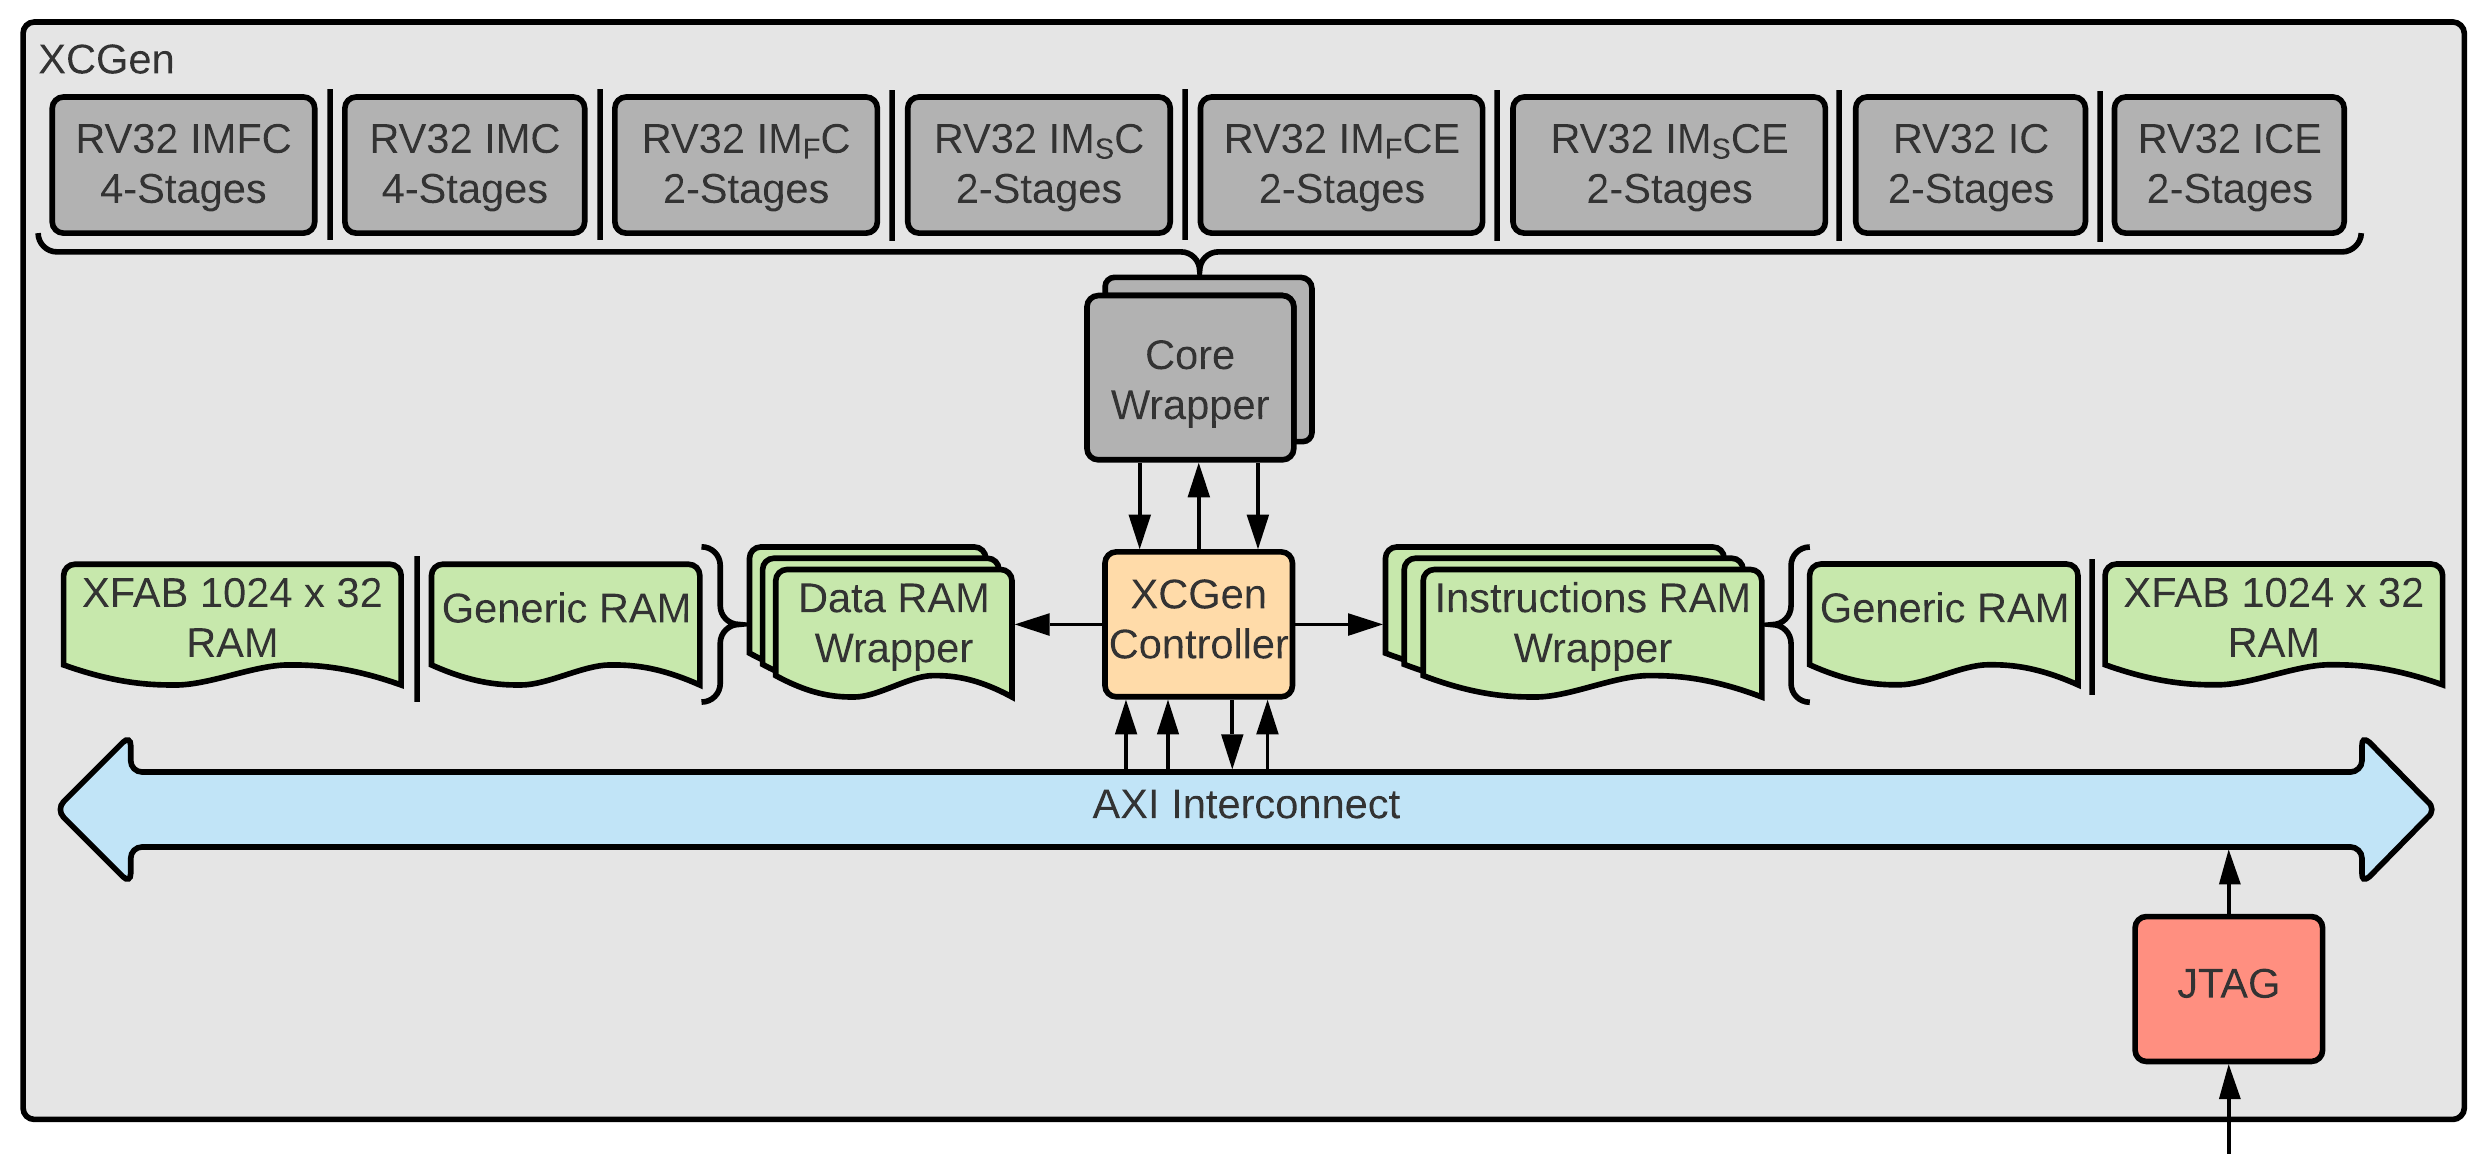
\includegraphics[width=\linewidth]{diagrams/XCGen2.png}
  \caption{Diagrama do XCGen.}
  \label{fig:top}
\end{figure}

\subsection{XCGen}
Através do uso dos parametros, é possível adicionar blocos ao SoC, como pode ser visto na imagem abaixo;
\begin{figure}[!htb]
  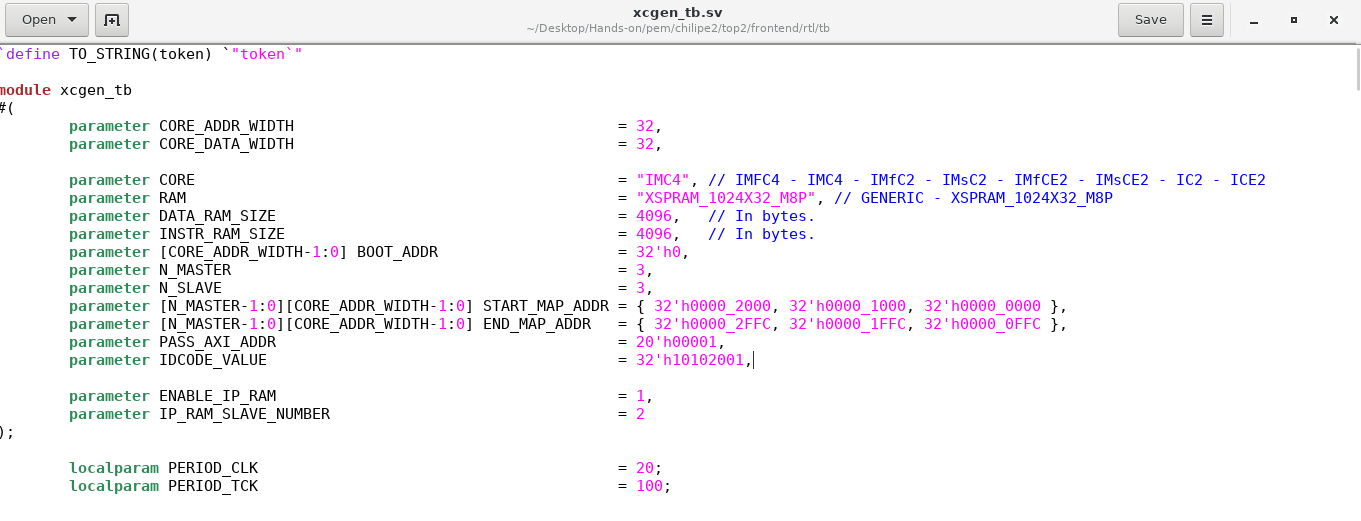
\includegraphics[width=\linewidth]{diagrams/tb.png}
  \caption{parametros do topo/tb.}
  \label{fig:top}
\end{figure}
\\
\begin{itemize}
  \item Alterando o número de mestres e escravos, é possível alterar a quantidade dos mesmos, no sistema;
  \item Possível alterar o tipo de processador(CORE);
  \item Possível alterar o tipo de memória(RAM)entre a  xfab e genérica(não sistetisável);
  \item atualmente é possível adicionar um IP generico, e definir o escravo(SLAVE) responsável pelo menos(ENABLE\_ IP\_RAM);
  \item É possível declarar qual dos escravos será responsável pelo novo IP(IP\_ RAM \_ SLAVE \_NUMBER);
  \item Total controle do mapa de memória do AXI(START/END\_ MAP \_ ADDR) ;
\end{itemize}

Na figura abaixo pode ser visto, como são adicionados novos blocos, através de generate, neste caso é o "generic\_ip":
\begin{figure}[!htb]
  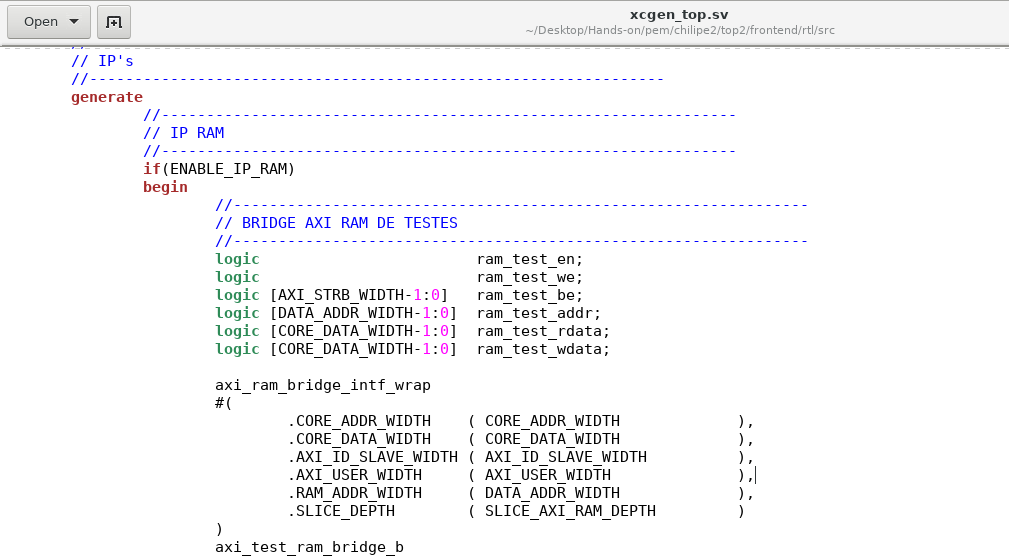
\includegraphics[width=\linewidth]{diagrams/ex_generate.png}
  \caption{Exemplo do uso de Generate.}
  \label{fig:top}
\end{figure}
\\
\subsection{CORE}
Core consiste no conjunto de processadores suportados pelo sistema, em comum eles possuem uma conexao direta as memórias de instrução e dados, e fazem o fetch, na memória de instruções, após o sinal fetch\_ enable\_i obter o valor "1";
A função do processador é executar instruções, utilizando o padrão da ISA risc\-v;

\subsection{JTAG}
O JTAG é responsável por fazer escrita e leitura nos registradores do SoC, ele faz isso através de uma entrada  e sáida serial, a qual o usuário tem acesso;
\begin{figure}[H]
  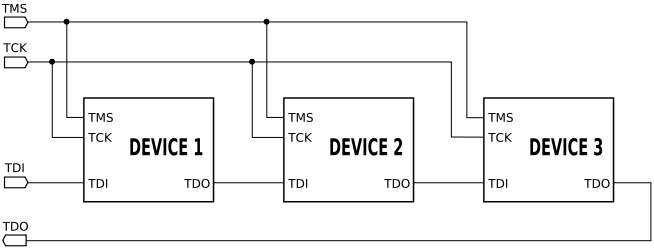
\includegraphics[width=\linewidth]{diagrams/jtag.png}
  \caption{jtag interface.}
  \label{fig:top}
\end{figure}

\subsection{AXI}
O AXI é responsável por conectar todos os mestres e escravos do sistema, através de uma interface em comum, e cada IP que não esteja neste padrão de sinais, possue uma bridge de tradução, para consolidar essa comunicação;
O AXI realiza transações através de um conjunto de handshakes  (valid,ready) para garantir que a informação chegou ao seu destino;
Possue 5 interfaces:

\begin{itemize}
  \item AW(address write): Consiste no endereço e seus sinais, onde se quer escrever uma informação;
  \item W(write):Consiste na informação a qual se quer escrever no endereço;
  \item B(response):Sinais de resposta a leitura;
  \item AR(address read):Consiste no endereço e seus sinais, onde se quer ler os dados;
  \item R(read):Consiste do dado a ser lido e seus sinais;
\end{itemize}
O AXI possue total controle para alterar o mapa de memória com os sinais:
\begin{itemize}
  \item start\_ add\_i : Endereço inicial de cada escravo(slave) do sistema;
  \item end\_ add\_i : Endereço final de cada escravo(slave) do sistema;
\end{itemize}
\begin{figure}[H]
  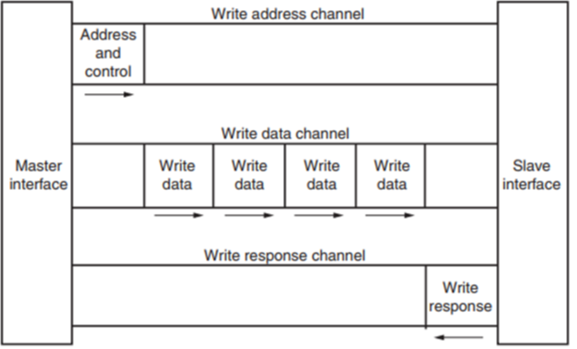
\includegraphics[width=\linewidth]{diagrams/axi comunication.png}
  \caption{Exemplo de transação axi.}
  \label{fig:top}
\end{figure}
\subsection{Tool chain}
É o a interface de software utilizada para geração de instruções em assembly(a ser interpretadas pelo core) através de uma linguágem de alto nível(c);
\begin{figure}[H]
  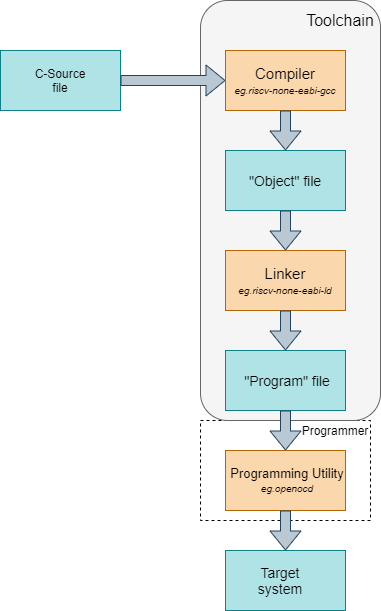
\includegraphics[width=\linewidth]{diagrams/toolchain.png}
  \caption{Fluxo da toolchain.}
  \label{fig:top}
\end{figure}
% section descricaofuncional (end)

\section{Hands-On} % (fold)
\label{sec:handson}
\subsection{Instalação}
Para iniciar, é necessário adquirir o bloco, que está localizado no git:
\begin{itemize}
  \item git clone user@10.75.211.9:/home/git/projects/pem
\end{itemize}
No seguinte branch:
\begin{itemize}
  \item git checkout chilipe2/int/dev/marcio
\end{itemize}


Após a aquisição do repositório, é necessário se dirigir a pasta na qual está contido o makefile responsável por instalar a toolchain:
\begin{itemize}
  \item cd pem/chilipe2/top2/frontend/software/toolchain\_openocd;
\end{itemize}
Após chegar no destino, é necessário rodar todas as linhas do makefile e para isso é obrigatório que o usuário tenha acesso de administrador, que no caso do Centos é o comando "sudo".
\begin{figure}[H]
  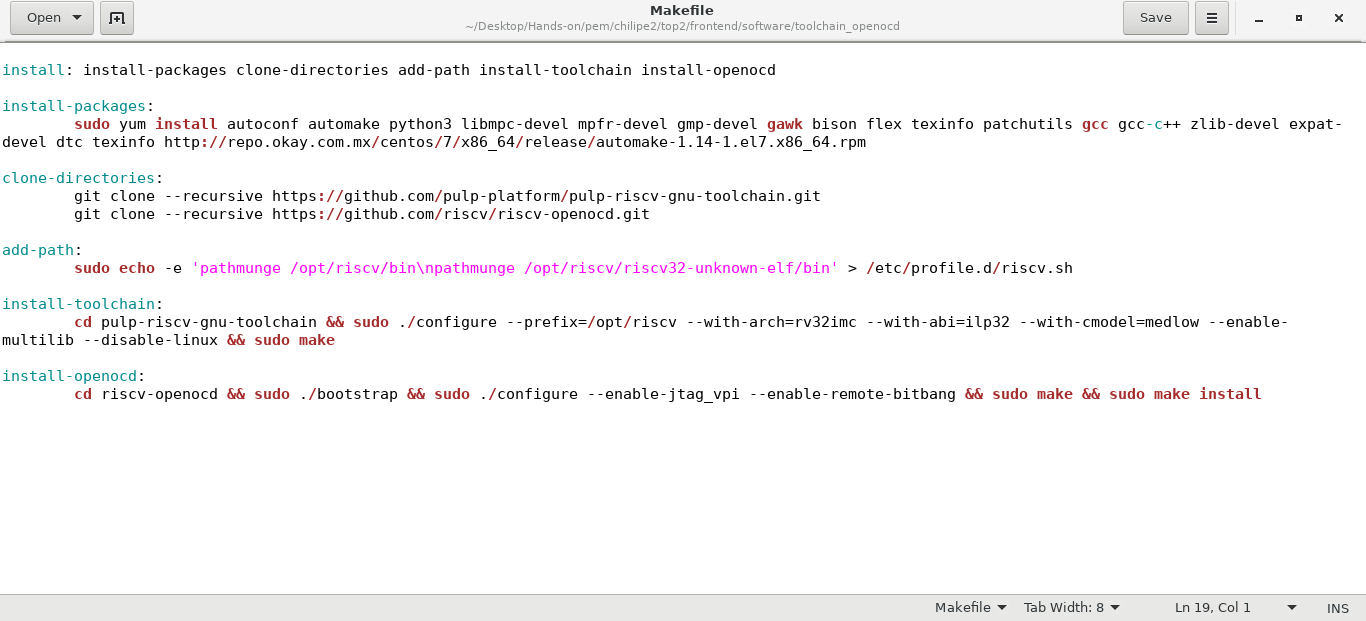
\includegraphics[width=\linewidth]{diagrams/makefile1.png}
  \caption{makefile.}
  \label{fig:top}
\end{figure}
Para rodar o makefile, recomendo não utilizar o "make install" e ir instalando linha por linha, pois pode ocorrer alguns erros; Na hora que eu rodei, deu erro na busca do repositório do openocd e do add-path, porém consegui rodar tudo no final, mesmo com esses erros.
\\	
Alguns dos comandos, podem levar até uma hora para serem executados, como é o caso dos comandos "install".


\subsection{Execução}
\par 1.Apos a instalação da toolchain, se desloque para a pasta:

\begin{itemize}
  \item cd pem/chilipe2/top2/frontend/workspace/src;
\end{itemize}

\par 2.Lá haverá um arquivo nomeado de test.c, no qual será necessário colocar o código que se deseja ser colocado no SoC.
\\
Para o propósito deste teste, um código estará contido abaixo:
\begin{lstlisting}
#define INIT_ADDR_INSTR_RAM 0x00000000
#define INIT_ADDR_DATA_RAM  0x00001000
#define INIT_ADDR_IP_RAM    0x00002000

int main()
{
	*(volatile int*) (INIT_ADDR_DATA_RAM + 0x00000000) = 0x00000030;
	*(volatile int*) (INIT_ADDR_DATA_RAM + 0x00000004) = 0x00000028;
	*(volatile int*) (INIT_ADDR_DATA_RAM + 0x00000008) = 0x00000015;
	*(volatile int*) (INIT_ADDR_DATA_RAM + 0x0000000C) = 0x00000022;
	*(volatile int*) (INIT_ADDR_DATA_RAM + 0x00000010) = 0x00000018;
	*(volatile int*) (INIT_ADDR_DATA_RAM + 0x00000014) = 0x0000004B;
	*(volatile int*) (INIT_ADDR_DATA_RAM + 0x00000018) = 0x0000004E;
	*(volatile int*) (INIT_ADDR_DATA_RAM + 0x0000001C) = 0x00000058;
	*(volatile int*) (INIT_ADDR_DATA_RAM + 0x00000020) = 0x00000004;
	*(volatile int*) (INIT_ADDR_DATA_RAM + 0x00000024) = 0x0000002B;
	*(volatile int*) (INIT_ADDR_DATA_RAM + 0x00000028) = 0x00000039;
	*(volatile int*) (INIT_ADDR_DATA_RAM + 0x0000002C) = 0x00000040;
	*(volatile int*) (INIT_ADDR_DATA_RAM + 0x00000030) = 0x00000001;
	*(volatile int*) (INIT_ADDR_DATA_RAM + 0x00000034) = 0x00000030;
	*(volatile int*) (INIT_ADDR_DATA_RAM + 0x00000038) = 0x00000038;
	*(volatile int*) (INIT_ADDR_DATA_RAM + 0x0000003C) = 0x00000002;
	*(volatile int*) (INIT_ADDR_DATA_RAM + 0x00000040) = 0x00000059;
	*(volatile int*) (INIT_ADDR_DATA_RAM + 0x00000044) = 0x0000003D;
	*(volatile int*) (INIT_ADDR_DATA_RAM + 0x00000048) = 0x00000000;
	*(volatile int*) (INIT_ADDR_DATA_RAM + 0x0000004C) = 0x00000009;
	*(volatile int*) (INIT_ADDR_DATA_RAM + 0x00000050) = 0x00000047;
	*(volatile int*) (INIT_ADDR_DATA_RAM + 0x00000054) = 0x0000002D;
	*(volatile int*) (INIT_ADDR_DATA_RAM + 0x00000058) = 0x0000005B;
	*(volatile int*) (INIT_ADDR_DATA_RAM + 0x0000005C) = 0x00000021;
	*(volatile int*) (INIT_ADDR_DATA_RAM + 0x00000060) = 0x00000005;
	*(volatile int*) (INIT_ADDR_DATA_RAM + 0x00000064) = 0x0000005E;
	*(volatile int*) (INIT_ADDR_DATA_RAM + 0x00000068) = 0x0000003E;
	*(volatile int*) (INIT_ADDR_DATA_RAM + 0x0000006C) = 0x00000047;
	*(volatile int*) (INIT_ADDR_DATA_RAM + 0x00000070) = 0x00000020;
	*(volatile int*) (INIT_ADDR_DATA_RAM + 0x00000074) = 0x00000058;
	*(volatile int*) (INIT_ADDR_DATA_RAM + 0x00000078) = 0x00000013;
	*(volatile int*) (INIT_ADDR_DATA_RAM + 0x0000007C) = 0x00000042;
	*(volatile int*) (INIT_ADDR_DATA_RAM + 0x00000080) = 0x00000023;
	*(volatile int*) (INIT_ADDR_DATA_RAM + 0x00000084) = 0x00000023;
	*(volatile int*) (INIT_ADDR_DATA_RAM + 0x00000088) = 0x0000005A;
	*(volatile int*) (INIT_ADDR_DATA_RAM + 0x0000008C) = 0x0000001C;
	*(volatile int*) (INIT_ADDR_DATA_RAM + 0x00000090) = 0x00000009;
	*(volatile int*) (INIT_ADDR_DATA_RAM + 0x00000094) = 0x00000005;
	*(volatile int*) (INIT_ADDR_DATA_RAM + 0x00000098) = 0x0000000D;
	*(volatile int*) (INIT_ADDR_DATA_RAM + 0x0000009C) = 0x0000003C;
	*(volatile int*) (INIT_ADDR_DATA_RAM + 0x000000A0) = 0x00000032;
	*(volatile int*) (INIT_ADDR_DATA_RAM + 0x000000A4) = 0x00000010;
	*(volatile int*) (INIT_ADDR_DATA_RAM + 0x000000A8) = 0x0000002D;
	*(volatile int*) (INIT_ADDR_DATA_RAM + 0x000000AC) = 0x00000020;
	*(volatile int*) (INIT_ADDR_DATA_RAM + 0x000000B0) = 0x0000002D;
	*(volatile int*) (INIT_ADDR_DATA_RAM + 0x000000B4) = 0x00000055;
	*(volatile int*) (INIT_ADDR_DATA_RAM + 0x000000B8) = 0x00000049;
	*(volatile int*) (INIT_ADDR_DATA_RAM + 0x000000BC) = 0x00000048;
	*(volatile int*) (INIT_ADDR_DATA_RAM + 0x000000C0) = 0x0000005C;
	*(volatile int*) (INIT_ADDR_DATA_RAM + 0x000000C4) = 0x0000001A;
	*(volatile int*) (INIT_ADDR_DATA_RAM + 0x000000CC) = 0x00000032; 

	int l = 1;
	while(l)
	{
		int k, j, aux;

		for (k = *(volatile int*) (INIT_ADDR_DATA_RAM + 0x000000CC) - 1; k > 0; k--)
		{
			for (j = 0; j < k; j++)
			{
				if (*(volatile int*) (INIT_ADDR_DATA_RAM + (j * 4)) > *(volatile int*) (INIT_ADDR_DATA_RAM + ((j + 1) * 4)))
				{
					*(volatile int*) (INIT_ADDR_INSTR_RAM + 0x00000FA0)   = *(volatile int*) (INIT_ADDR_DATA_RAM + (j * 4));
					*(volatile int*) (INIT_ADDR_DATA_RAM + (j * 4))       = *(volatile int*) (INIT_ADDR_DATA_RAM + ((j + 1) * 4));
					*(volatile int*) (INIT_ADDR_DATA_RAM + ((j + 1) * 4)) = *(volatile int*) (INIT_ADDR_INSTR_RAM + 0x00000FA0);
				}
			}
		}
	}
}
\end{lstlisting}

Explicando brevemente:
\\
A primeira sessão onde tem "init addr" é responsável por gerar os valores iniciais da memória de dados, os quais vão ser organizados.
\\
A segunda sessão, a partir do "while", representa um bubble sort, um algoritmo de organização,o qual será carregado na memória de instruções. Onde vai ser lido pelo core e executar a organização da memória de dados. 
\\

\par 3.Após o código ser colocado, utilize o seguinte comando para voltar uma pasta:

\begin{itemize}
  \item cd ..
\end{itemize}
\par 4.Aqui temos um Makefile, abra o terminal e digite:

\begin{itemize}
  \item make all
\end{itemize}

\par 5.Após executar do comando, 3 arquivos aparecerão na pasta:

\begin{itemize}
  \item cd pem/chilipe2/top2/frontend/rtl/tb
\end{itemize}

\begin{figure}[H]
  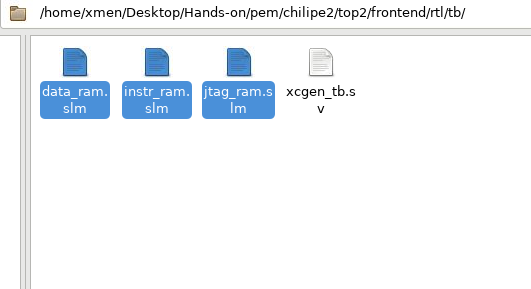
\includegraphics[width=\linewidth]{diagrams/pastatb.png}
  \caption{Arquivos na pasta tb.}
  \label{fig:top}
\end{figure}

\par 6.O arquivo é chamado jtag\_ ram\_slm , o qual vai ser lido pelo testbench, e o colocará na entrada do jtag, simulando uma interface externa e através disso, escrever nas memórias de instruções e de dados, as informações em hexadecimal, do que foi feito em C.
\\
\par 7.Agora, para a compilação do código, se dirija para :

\begin{itemize}
  \item cd ..
  \item cd ..
  \item cd scripts/rlsim
\end{itemize}

\par 8;Onde será executado os seguintes comandos:

\begin{itemize}
  \item cds
  \item make
  \item make waves
\end{itemize}

\par 9.Isto abrirá uma janela no programa "simvision" na qual será possível observer o que ocorre durante todo processo, desde a escrita nas memórias de dados e instruções através do JTAG, até a execução do código(bubble sort) pelo processador, e a organização da memória de dados através deste processo.
\\
\subsection{Faça seu teste}
Caso se deseja realizar outro teste, com diferentes endereços de memórias, é necessário alterar as informações no linker, que pode ser encontrado em:

\begin{itemize}
  \item cd pem/chilipe2/top2/frontend/workspace/tools/xcgen/ld;
\end{itemize}

Caso se deseja apenas alterar o código em C, basta alterar o código do arquivo test.c e realizar o mesmos passos (apartir do 3.)citados na sessão anterior.
\\
% subsection Hands-On (end)

%\section{Informação extra} % (fold)
\label{sec:informação_extra}

% section informação_extra (end)

%\section{Informação de inicialização} % (fold)
\label{sec:informação_de_inicialização}

% section informação_de_inicialização (end)

%\section{Informação de aplicação} % (fold)
\label{sec:informação_de_aplicação}

% section informação_de_aplicação (end)

\end{document}
